\documentclass[11pt,a4paper]{article}

\usepackage[T1]{fontenc}
\usepackage[utf8]{inputenc}
\usepackage[margin=25mm]{geometry}
\usepackage{graphicx}
\usepackage{booktabs}
\usepackage{amsmath}
\usepackage[hidelinks]{hyperref}
\usepackage{microtype}

\graphicspath{{assets/}}
\setlength{\parindent}{0pt}
\setlength{\parskip}{6pt}
\newcommand{\code}[1]{\nolinkurl{#1}}
\setlength{\emergencystretch}{2em}

\title{Pool Ball Detection and Recognition\\[4pt]
       \large Computer Vision Assignment --- Draft Report}
% Replace this author field before submission.
\author{Author name and student number}
\date{27 October 2026}

\begin{document}
\maketitle

\begin{abstract}
This project implements a C++17 and OpenCV pipeline for detecting pool balls,
classifying their type, and estimating their number from colour. Detection uses
table masking, the circular Hough transform, and geometric filtering near
pockets. Recognition uses K-means colour segmentation, with an optional
connected-component analysis (CCA) stage. In the saved six-image validation
results, detection achieves an aggregate F1 score of 0.940. Among 86 matched
and analysed balls, the baseline correctly classifies 76 types and 67 numbers;
the CCA variant correctly classifies 73 types and 64 numbers. These figures
describe the saved experiment outputs rather than a new evaluation run.
\end{abstract}

\section{Task and dataset}
The system processes a photograph of a pool table and produces detected ball
centres, predicted types, and predicted numbers. The type categories are White,
Solid, and Striped. Number 0 denotes the cue ball, numbers 1--8 are solids, and
numbers 9--15 are stripes. A predicted number of $-1$ denotes an unknown result.

\code{AllBalls.jpeg} is used for tuning and inspecting colour clusters.
\code{Table1.jpeg} through \code{Table6.jpeg} form the validation image set.
The saved detection results contain 90 annotated balls across these six images.
Ground-truth positions and numbers are loaded from
\code{data/ground_truth/BallLocations.csv}. Actual numbers are used for matching
and scoring; they are not inputs to the number classifier.

\section{Method}
\subsection{Detection and geometric filtering}
Pixels outside a manually specified table quadrilateral are masked out. The
image is converted to grayscale and smoothed with a $5\times5$ Gaussian filter
with standard deviation 1.5. Circular Hough detection then proposes ball centres
and radii. Table~\ref{tab:parameters} lists the configured detection parameters.

\begin{table}[htbp]
\centering
\caption{Configured detection and evaluation parameters.}
\label{tab:parameters}
\begin{tabular}{lr}
\toprule
Parameter & Value \\
\midrule
Hough accumulator resolution ratio & 1.5 \\
Minimum centre separation (original-image pixels) & 18 \\
Hough edge threshold / accumulator threshold & 75 / 35 \\
Minimum / maximum radius (original-image pixels) & 15 / 30 \\
Transformed table size (pixels) & $1434\times683$ \\
Pocket exclusion radius (transformed pixels) & 25 \\
Ground-truth matching tolerance (transformed pixels) & 15 \\
\bottomrule
\end{tabular}
\end{table}

A perspective transformation maps detected centres into table coordinates.
Candidates within 25 transformed pixels of an approximate pocket centre are
removed. The retained circles remain in original-image coordinates for cropping
and drawing. Ground-truth matching is performed in transformed coordinates.

\begin{figure}[htbp]
\centering
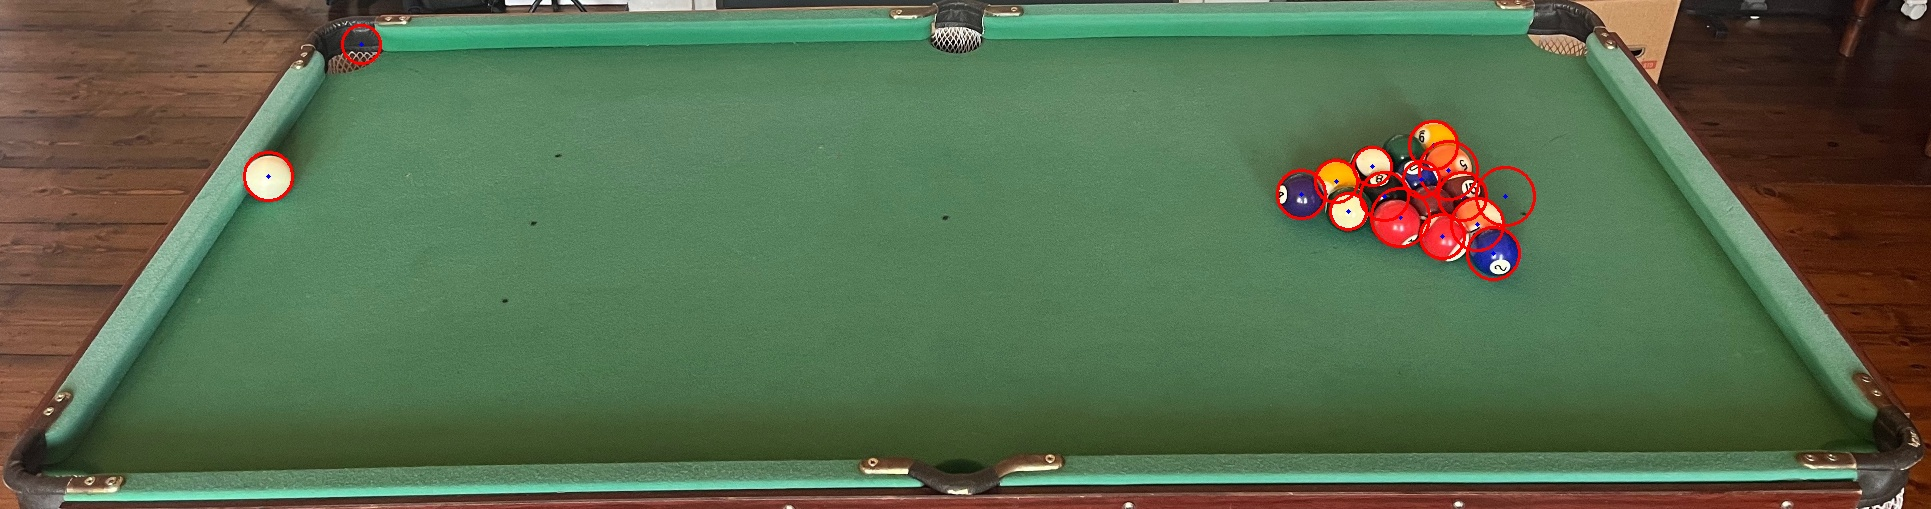
\includegraphics[width=0.88\linewidth]{table1-detection.jpeg}
\caption{Saved detection overlay for Table1. This image illustrates the output;
quantitative detection counts are reported in Table~\ref{tab:detection}.}
\label{fig:detection}
\end{figure}

\subsection{Ball extraction and K-means segmentation}
Each detected ball is cropped from the original colour image and assigned a
circular binary mask. Only pixels inside this mask are clustered. K-means uses
three-dimensional BGR samples; HSV values are computed from the resulting
cluster colours for subsequent analysis. The demo compares $K=2,3,4,5$, while
the configured recognition pipeline uses $K=2$.

Each cluster stores its mask, percentage of the ball area, BGR colour, and HSV
colour. Cluster percentages are computed relative to the circular ROI, and
clusters are sorted by decreasing area. Diagnostic grids combine the original
crop, segmented images, and cluster masks with labels.

\begin{figure}[htbp]
\centering
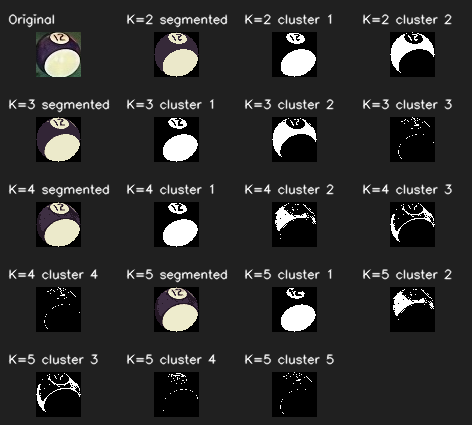
\includegraphics[width=0.60\linewidth]{kmeans-example.png}
\caption{Saved AllBalls diagnostic grid for candidate 6, showing the original
crop and the segmentation and masks for $K=2$ through $K=5$.}
\label{fig:kmeans}
\end{figure}

\subsection{Type classification}
For each cluster, saturation $S$ and brightness $V$ determine its category.
A cluster is light when $V\geq170$ and $S\leq165$, dark when $V\leq90$, and
coloured otherwise. The classifier sums the area percentages in each category.
The decision rules are applied in the following order:
\begin{enumerate}
\item White if at least 85\% of the ball is light.
\item Solid if the combined coloured and dark percentage is at least 70\%.
\item Striped if both light and non-light regions are present.
\item Unknown if no preceding rule applies.
\end{enumerate}
The black ball remains a Solid at this stage.

The optional CCA classifier starts with this baseline prediction. It examines
light and non-light connected components, excluding components smaller than
2\% of the ball area. It also measures light coverage within a boundary band
obtained by eroding the circular ROI mask. Additional rules use these features
to revise the predicted type. A stricter White rule does not reject all baseline
White predictions: when no CCA rule applies, the baseline prediction is retained.

\subsection{Number recognition}
Number recognition follows type recognition and reuses the segmentation. White
maps to the cue ball, number 0. For solids and stripes, the largest eligible
non-light cluster supplies the body colour; clusters smaller than 2\% are
ignored. Experimental HSV rules identify yellow, blue, red, purple, orange,
green, or maroon. The corresponding solid numbers are 1--7, and stripes add 8.
A dark, low-saturation body cluster can identify number 8 when the predicted type
is Solid. Red and maroon are separated using brightness. Unsupported colours
return $-1$ rather than forcing a number prediction.

The application keeps detection, type recognition, and number recognition as
three separate stages. It saves type-labelled and number-labelled images, along
with CSV files containing the predictions.

\section{Evaluation and saved results}
\subsection{Detection}
Detections are matched one-to-one to annotated centres within the configured
15-pixel tolerance. The matching procedure maximises the number of valid
matches; it does not globally minimise localisation distance. Precision, recall,
and F1 are computed as
\[
 P=\frac{TP}{TP+FP},\qquad
 R=\frac{TP}{TP+FN},\qquad
 F_1=\frac{2TP}{2TP+FP+FN}.
\]
\begin{table}[htbp]
\centering
\caption{Saved detection results. The total row uses aggregate counts.}
\label{tab:detection}
\begin{tabular}{lrrrrrr}
\toprule
Image & TP & FP & FN & Precision & Recall & F1 \\
\midrule
Table1 & 14 & 2 & 2 & 0.875 & 0.875 & 0.875 \\
Table2 & 16 & 2 & 0 & 0.889 & 1.000 & 0.941 \\
Table3 & 15 & 0 & 1 & 1.000 & 0.938 & 0.968 \\
Table4 & 14 & 1 & 1 & 0.933 & 0.933 & 0.933 \\
Table5 & 14 & 1 & 0 & 0.933 & 1.000 & 0.966 \\
Table6 & 13 & 1 & 0 & 0.929 & 1.000 & 0.963 \\
\midrule
Total & 86 & 7 & 4 & 0.925 & 0.956 & 0.940 \\
\bottomrule
\end{tabular}
\end{table}


\subsection{Recognition}
Type and number correctness are evaluated separately. The number classifier is
called once with the baseline type and once with the CCA type. Unknown number
predictions count as incorrect. Recognition accuracy below is conditional on
the 86 matched and successfully analysed detections; unmatched detections are
excluded from the recognition loop.
\begin{table}[htbp]
\centering
\small
\caption{Correct recognition counts among matched and analysed balls. B: baseline; C: CCA. Percentages in the total row are conditional accuracies.}
\label{tab:recognition}
\begin{tabular}{lrrrrr}
\toprule
Image & Analysed & Type B & Type C & Number B & Number C \\
\midrule
Table1 & 14 & 8 & 8 & 6 & 6 \\
Table2 & 16 & 15 & 14 & 13 & 12 \\
Table3 & 15 & 14 & 13 & 14 & 13 \\
Table4 & 14 & 14 & 13 & 13 & 12 \\
Table5 & 14 & 14 & 14 & 11 & 11 \\
Table6 & 13 & 11 & 11 & 10 & 10 \\
\midrule
Total & 86 & 76 & 73 & 67 & 64 \\
Accuracy & --- & 88.4\% & 84.9\% & 77.9\% & 74.4\% \\
\bottomrule
\end{tabular}
\end{table}


These tables are snapshots of the existing CSV outputs. They are not updated
automatically when the application is rebuilt or when LaTeX is compiled. The
recognition source CSVs contain an extra empty trailing field in each row; this
was ignored after checking that the named correctness flags agreed with the
stored predictions and ground truth. The numerical columns were not shifted.

\section{Discussion and limitations}
CCA does not improve the aggregate results in the saved validation outputs:
both type and number accuracy are lower than the baseline. Its additional
spatial rules should therefore be assessed per image and per error case before
being adopted in the main application.

The number classifier uses experimental thresholds chosen for the current image
set. Illumination affects brightness and saturation, particularly for dark blue,
purple, green, and maroon balls. The red--maroon brightness split is especially
sensitive to shadows. A type error can also change a correct colour estimate
into the wrong numbered ball by applying the solid/stripe offset incorrectly.

Fixed table corners, radius ranges, and pocket locations restrict the current
pipeline to a similar camera view. Pocket filtering may remove a genuine ball
close to a pocket. Future experiments should examine colour normalisation,
additional views and lighting conditions, and error cases for each class.
Development and tuning on the validation images would also need to be disclosed;
these results should not be described as an independent held-out test without
checking that separation.

\section{Reproducibility and report status}
The implementation uses C++17, OpenCV 4, and CMake. From the project root,
\code{cmake --build build-local} builds the application. Menu 8 runs the
AllBalls K-means experiment; menu 9 runs recognition validation; menu 4 runs
detection validation; menu 1 runs the interactive three-stage application.

This is an editable draft based on the local implementation and saved outputs.
Before submission, replace the author field, check the assignment requirements,
add the required literature references, and refresh the result tables after any
changes to the classifier or experiment settings. The copied example figures
and table sources are included within the report folder so the document can be
compiled independently of the application output directory.

\end{document}
